\documentclass[10pt]{article}
\usepackage[margin=1.7cm]{geometry}
\usepackage{libertine}
\usepackage{amsmath}
\usepackage[version=4]{mhchem}
\usepackage{xcolor}
\usepackage{tikz}
\usepackage{enumitem}
\usetikzlibrary{arrows.meta, positioning}
\pagestyle{empty}
\setlength{\parindent}{0pt}
\setlength{\parskip}{0.5em}

\definecolor{accent}{HTML}{2E7D4F}
\definecolor{panel}{HTML}{EEF6F0}

\newcommand{\heading}[1]{{\bfseries\color{accent} #1}}

\begin{document}

{\LARGE\bfseries\color{accent} Molecular Biology Notes}\\[0.1em]
{\large Lecture 7: glycolysis, ATP hydrolysis, and pathway regulation}

\vspace{0.5em}
\heading{1. ATP hydrolysis}

The energy released by cellular reactions is stored and transported mainly as
adenosine triphosphate. Hydrolysis of the terminal phosphate anhydride bond is
exergonic:
\[
  \ce{ATP + H2O -> ADP + Pi}, \qquad \Delta G^{\circ\prime} \approx -30.5\ \text{kJ/mol}.
\]
This reaction is coupled to otherwise unfavorable steps throughout metabolism,
most notably the first two steps of glycolysis.

\heading{2. The committed step of glycolysis}

Phosphofructokinase-1 (PFK-1) catalyzes the committed step, phosphorylating
fructose-6-phosphate at the cost of one ATP:
\[
  \ce{Fructose-6-phosphate + ATP ->[PFK-1] Fructose-1,6-bisphosphate + ADP}.
\]
PFK-1 is allosterically inhibited by high \ce{ATP} and citrate, and activated
by \ce{AMP} and fructose-2,6-bisphosphate, making it the primary control point
for flux through the pathway.

\heading{3. Substrate-level phosphorylation}

Later in glycolysis, phosphoglycerate kinase and pyruvate kinase generate ATP
directly from a substrate rather than from the electron transport chain:
\[
  \ce{1,3-Bisphosphoglycerate + ADP ->[PGK] 3-Phosphoglycerate + ATP},
\]
\[
  \ce{Phosphoenolpyruvate + ADP ->[Pyruvate\ kinase] Pyruvate + ATP}.
\]
Overall, one glucose molecule yields a net two ATP and two NADH through the
ten reactions of glycolysis.

\vspace{0.4em}
\noindent
\begin{minipage}[t]{0.56\textwidth}
\heading{4. Pathway overview}

\vspace{0.5em}
\begin{center}
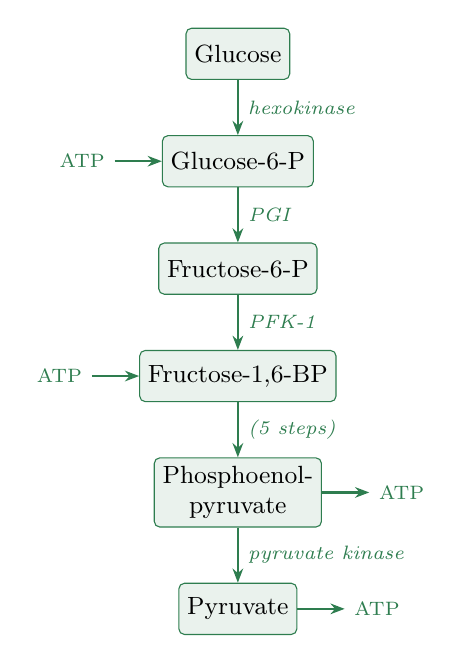
\begin{tikzpicture}[
    node distance=7mm and 9mm,
    every node/.style={font=\small},
    met/.style={draw=accent, fill=accent!10, rounded corners=2pt,
      minimum height=6.5mm, align=center, inner sep=3pt},
    enz/.style={font=\scriptsize\itshape, accent},
    arr/.style={-{Stealth[length=1.8mm]}, accent, thick}
  ]
  \node[met] (glu)  {Glucose};
  \node[met, below=of glu] (g6p) {Glucose-6-P};
  \node[met, below=of g6p] (f6p) {Fructose-6-P};
  \node[met, below=of f6p] (f16bp) {Fructose-1,6-BP};
  \node[met, below=of f16bp] (pep) {Phosphoenol-\\pyruvate};
  \node[met, below=of pep] (pyr) {Pyruvate};

  \draw[arr] (glu)   -- (g6p)   node[midway, enz, right] {hexokinase};
  \draw[arr] (g6p)   -- (f6p)   node[midway, enz, right] {PGI};
  \draw[arr] (f6p)   -- (f16bp) node[midway, enz, right] {PFK-1};
  \draw[arr] (f16bp) -- (pep)   node[midway, enz, right] {(5 steps)};
  \draw[arr] (pep)   -- (pyr)   node[midway, enz, right] {pyruvate kinase};

  \node[left=6mm of g6p, accent, font=\scriptsize] (atp1) {ATP};
  \draw[arr] (atp1) -- (g6p);
  \node[left=6mm of f16bp, accent, font=\scriptsize] (atp2) {ATP};
  \draw[arr] (atp2) -- (f16bp);
  \node[right=6mm of pep, accent, font=\scriptsize] (atp3) {ATP};
  \draw[arr] (pep) -- (atp3);
  \node[right=6mm of pyr, accent, font=\scriptsize] (atp4) {ATP};
  \draw[arr] (pyr) -- (atp4);
\end{tikzpicture}
\end{center}
\end{minipage}%
\hfill
\begin{minipage}[t]{0.4\textwidth}
\heading{5. Regulation summary}

\vspace{0.4em}
\begin{itemize}[leftmargin=1.1em]
  \item[--] \textbf{Hexokinase}: inhibited by its own product, glucose-6-P.
  \item[--] \textbf{PFK-1}: the master regulator, inhibited by ATP and
    citrate, activated by AMP and F2,6BP.
  \item[--] \textbf{Pyruvate kinase}: inhibited by ATP and alanine,
    activated by fructose-1,6-BP (feed-forward).
\end{itemize}

\vspace{0.6em}
{\small Together these three irreversible steps make glycolysis responsive
to the cell's energy charge without needing to regulate every enzyme in the
pathway.}
\end{minipage}

\end{document}
